\section{Alternative Ideas}



%:::\revisit[Do we still need the paragraph below? It is a detailed example on how this paper might provide guidance on selection an appropriate model for an application] ::Daniel to check it later
% also the importance of constant factor approximation
% In applications, it is preferable to formulate a real-world problem as a computational problem solvable in polynomial time. However, when the application requires a more complex model whose a global optimum is intractable, it is often satisfactory to solve the problem to a desired relative accuracy in the objective, \ie, reaching the optimum within a given ratio. Indeed, such algorithms exist such as the well-known Potts model can be approximated by alpha-expansion \cite{boykov2001approximate} within a constant factor of 2. In structural learning \cite{finley2008training} for example, it is acceptable to have a constant factor approximation algorithm for the inference oracle, also an instance of energy minimization, when efficient exact algorithms are not available. This is because the constant factor approximation for the inference oracle can yield a multiplicative bound on the learning objective, providing a relative guarantee for the quality of the learned parameters. In sum, the solution quality of structural learning depends on the approximation guarantees of the energy minimization subroutine. It is shown in cite{another eccv submission} that when such an efficient subroutine is impossible even in terms of constant ratio approximation, we should reformulate the learning objective to make the learning problem tractable.

%::: move to later... Therefore, algorithm designers should not expect to prove a reasonable approximation ratio guarantee for their algorithms on general energy minimization algorithms.

% When terms depending on three or more variables are present in~\eqref{eq:1}, the problem is known as {\em higher-order}\footnote{There is a discrepancy in the literature on whether to refer to~\eqref{eq:1} as first or second order. It has first order interactions when viewed as a Markov model. On the other hand, in QPBO it is a second order polynomial in $x$.}. We focus primarily on the pairwise case but notate results that hold for higher order as well. In the higher order pseudo-Boolean case, the problem is known as general pseudo-Boolean optimization or as $0$-$1$ polynomial programming.


% \paragraph{Complexity Classes} For decision problems, class NP (nondeterministic polynomial time) includes problems whose solution can be verified in polynomial time. Analogously for optimization problems, class NPO (NP-optimization) is introduced for problems whose solution feasibility can be verified in polynomial time. Its formal definition is given in \Section{sec:complexitytheory}. 
% %::: section does not exist
% The NP-hardness of an optimization problem means it is at least as hard as the hardest decision problem in the class NP. These concepts are illustrated in \Figure{fig:Classes-P-NP}.

% \begin{figure}[t]
% \begin{center}
% \resizebox{0.9\linewidth}{!}{
% \begin{tabular}{cc}
% \begin{tabular}{c}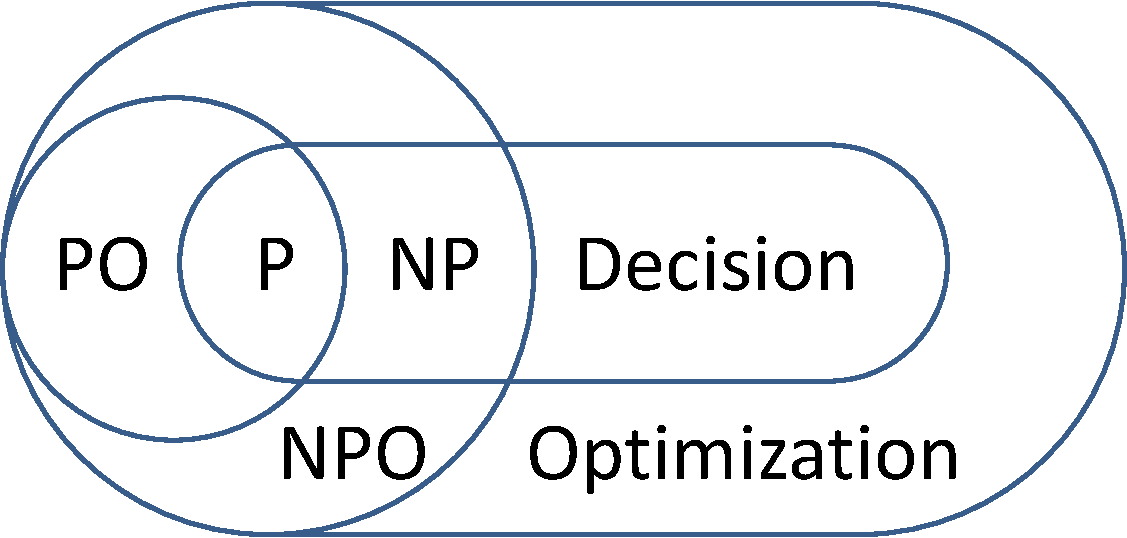
\includegraphics[width=0.43\linewidth]{figure/Classes-P-NP-crop.pdf}\end{tabular}%
% \ \ 
% 	 \begin{tabular}{c}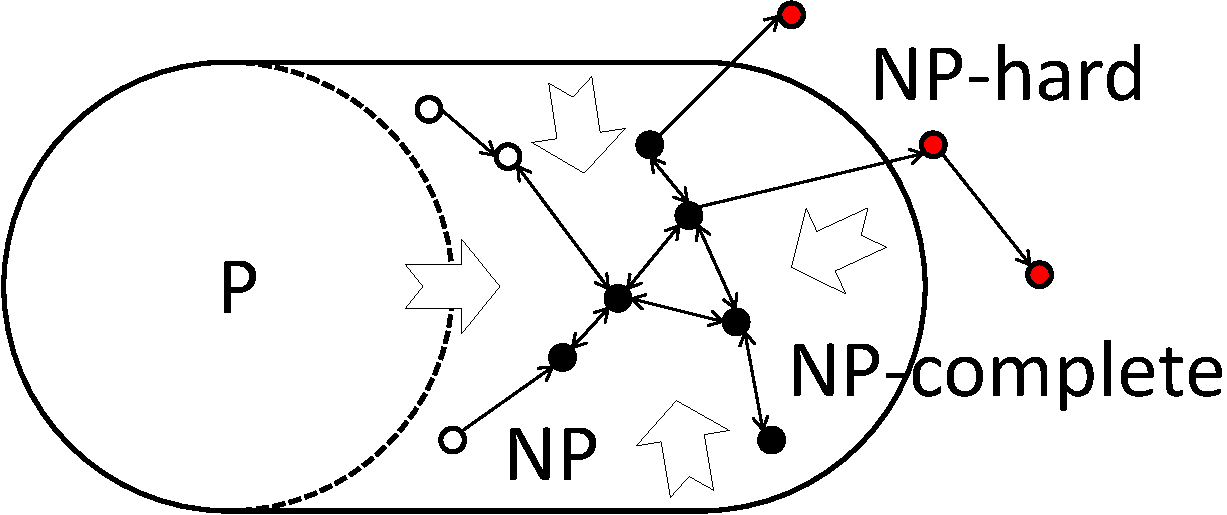
\includegraphics[width=0.5\linewidth]{figure/Classes-NP-hard-crop.pdf}\\[5pt]
% 	\end{tabular}%
% 	\end{tabular}
% 	}
% \end{center}
%   \caption{Left: relation of complexity classes between decision and optimization problems. Optimization problems ``contain'' decision problems since any decision problem can be cast as an optimization over the set $\{$yes, no$\}$. If not clear from the picture, P $\subseteq$ NP, P $\subseteq$ PO and NP $\subseteq$ NPO. Right: arrows indicate that a problem can be reduced to other problem in polynomial time. %All NP problems can be reduced to NP-complete problems. If a problem is such that an NP-complete problem reduces to it, 
% % I am not sure you need to include the right part of the figure.  Anyone reading the paper should understand the basic concept of a reduction.
% NP-hard class contains NP-complete problems and all problems (not necessarily decision) that are at least as hard (to which an NP-complete problem, and thus all problems in NP, may be reduced).
% }
% \label{fig:Classes-P-NP}
% \end{figure}

Suggestions for the right part figure 2 (update: already merged with figure 1 now):

Three ways to improve it:

1. Keep the idea of using dots as problems and edges as reductions, but makes solid arrows larger and replace hollow arrows with a dotted boundary for NP-complete problems.

2. Actually, wikipedia has a nice figure explaining this problem:
\par
\url{https://en.wikipedia.org/wiki/P_versus_NP_problem#/media/File:P_np_np-complete_np-hard.svg}
\par
We don't need to introduce reduction here for a) simplicity, b) avoid technical issues:
Karp reduction is used for reductions among decision problems while Turing reduction is used from decision problems to optimization problems. In other words, the typical reduction used for decision problems does not work for optimizaiton problems.

3. Just remove the right half of figure 2 as it is already something well explained on Wikipedia. We can resort to just text explanation.

---------------------------------------





   %Discrete energy minimization is an established work engine for performing inference in graphical models 
%   Discrete energy minimization is a recognized optimization problem, used to solve MAP inference in graphical models and closely related to several well-known combinatorial optimization problems.
%<<<<<<< Updated upstream
   %In this paper we give a comprehensive overview of subclasses solvable in polynomial time as well as subclasses admitting a constant factor approximation. We further contribute to the study of complexity by showing that general energy minimization is exp-APX-complete, meaning it is as hard as any optimization problem with a polynomial-time computable objective function and whose arbitrary feasible solution can be found in polynomial time, and the general problem cannot be approximated with a better then exponential factor. The result holds already in case of two labels, \ie, for quadratic pseudo-Boolean optimization. Further, we show that planar problem with 3 labels is exp-APX-complete as well.
%% \par
% \revisit[I think it might be better to keep the exponential factor as in previous version. "as hard as bla bla" is still vague to people without a sense of what is an optimization problem.]
%=======
%   In this paper we give a comprehensive overview of subclasses solvable in polynomial time as well as subclasses admitting a constant factor approximation. We further contribute to the study of complexity by showing that general energy minimization is exp-APX-complete, meaning that 
% 	it is NP-hard to approximate it with a subexponential ratio. %find a solution with energy within a subexponential (in the problem size) factor of the minimum.
%  %and cannot be approximated with a better then exponential factor. 
% The result holds already in case of two labels, \ie, for quadratic pseudo-Boolean optimization. Further, we show that planar problem with 3 labels is exp-APX-complete as well.
% \par
% %\revisit[I think it might be better to keep the exponential factor as in previous version. "as hard as bla bla" is still vague to people without a sense of what is an optimization problem.]
% %>>>>>>> Stashed changes
     
% \revisit[See ideas.tex for an alternative abstract that is tied closer to computer vision]


% Discrete energy minimization problem, which can be used to solve MAP inference for graphical models, is widely adopted in computer vision and machine learning. Despite many subclass problems are identified as NP-hard, they are still used to model real world applications. In this paper, we present a comprehensive overview of the computational complexity of subclass problems by arranging them on a finer complexity scale consisting of three major complexity classes --- PO, APX, exp-APX, corresponding to problems that are solvable, approximable, inapproximable in polynomially time. The connections of these subclass problems will also be analyzed. We hope this overview will aid researchers in designing new optimization algorithms
% and in selecting appropriate models for their applications. Moreover, we contribute two important additions to this overview by showing that general energy minimization and planar 3-label energy minimization are exp-APX-complete. This essentially mean that there cannot be any approximation algorithm with an approximation ratio better than an exponential function in the input size for these two problems. Therefore algorithm designers should not expect to prove a reasonable approximation ratio guarantee for their algorithms on these problems.


---------------------------

Previous version of the related works:


% NP-hardness has been shown for the MAP assignment of belief networks by~\citet{Cooper-90} and \citet{Shimony-94}. \citet{Abdelbar-98} has shown that approximating the MAP assignment is also NP-hard. However, there are substantial differences from our result.
% Belief networks have a probability density function $p(x)$ that factors according to a directed acyclic graph, \eg, as $p(x_1,x_2,x_3) = p(x_1 | x_2,x_3)p(x_2)p(x_3)$. %Using the relation $p(x) = \exp(-f(x))$, 
% %The negative logarithm of the pdf is then representable as a partially separable function of the form~\eqref{eq:1}. Maximization of the probability 
% For belief networks, finding the MAP assignment\footnote{Same as the most probable estimate (MPE).} in a Bayesian network is related to energy minimization~\eqref{eq:1} by letting $f(x) = -\log(p(x))$. The product is transformed into the sum and so, \eg, factor $p(x_1 | x_2,x_3)$ corresponds to term $f_{1,2,3}(x_1,x_2,x_3)$.
% %
% Note, factors of at most two variables, \eg, $p(x_1 | x_2)$, can form only a tree-structured model. % and therefore a Bayesian Network corresponding to a given energy may require higher order factors.
% %In the other direction, 
% Therefore, a Bayesian network corresponding to the pairwise energy~\eqref{eq:1} may require to use factors of order up to $|V|$. \revisit[this sentence is confusing] % in the Bayesian Network representation. 
% It is seen that while the general problems are convertible, fixed-parameter classes (such as order and graph restrictions) differ. In addition, approximation ratio for probabilities translates to an absolute approximation (an additive bound) for energies.


% \citet{Abdelbar-98} has shown that approximating the MAP assignment is also NP-hard. However, there are substantial differences from our result.

% are two neccessary conditions for the problem to be in PO. 
% more general means not only undirected graphical models,
% not only MAP inference, also marginal, partition function

% how to properly cite this?
% http://www.cs.huji.ac.il/project/PASCAL/index.php

% It is well-known that QPBO is NP-hard, since it generalizes such problems as maximum cut and maximum 2-satisfiability~\cite{Karp-72}. 
% These problems are also known to be APX-complete~\cite{Papadimitriou-91} (implies NP-hardness). Therefore, QPBO is APX-hard.
% %::: this does not flow very well.  This next text is not really related work.  It is more about our work.  Maybe better to just say "In this paper, we prove the stronger claim that QPBO is complete in exp-APX."
% Completeness in exp-APX is stronger. 
%::: suggest moving the following text to the section on the proof.
% In particular, it shows that such problems as general traveling salesman problem (TSP) can be reduced to QPBO while preserving approximation ratio in a linear fashion.

%:::\revisit[Consider finding a place to explicitly stating that BNs capture different families of distributions than energy minimization and thus they are used to model different problems]

% NP-hardness has been shown for the MAP assignment of belief networks by~\citet{Cooper-90} and \citet{Shimony-94}. \citet{Abdelbar-98} has shown that approximating the MAP assignment is also NP-hard. However, there are substantial differences from our result.
% Belief networks have a probability density function $p(x)$ that factors according to a directed acyclic graph, \eg, as $p(x_1,x_2,x_3) = p(x_1 | x_2,x_3)p(x_2)p(x_3)$. %Using the relation $p(x) = \exp(-f(x))$, 
% %The negative logarithm of the pdf is then representable as a partially separable function of the form~\eqref{eq:1}. Maximization of the probability 
% For belief networks, finding the MAP assignment\footnote{Same as the most probable estimate (MPE).} in a Bayesian network is related to energy minimization~\eqref{eq:1} by letting $f(x) = -\log(p(x))$. The product is transformed into the sum and so, \eg, factor $p(x_1 | x_2,x_3)$ corresponds to term $f_{1,2,3}(x_1,x_2,x_3)$.
% %
% Note, factors of at most two variables, \eg, $p(x_1 | x_2)$, can form only a tree-structured model. % and therefore a Bayesian Network corresponding to a given energy may require higher order factors.
% %In the other direction, 
% Therefore, a Bayesian network corresponding to the pairwise energy~\eqref{eq:1} may require to use factors of order up to $|V|$. \revisit[this sentence is confusing] % in the Bayesian Network representation. 
% It is seen that while the general problems are convertible, fixed-parameter classes (such as order and graph restrictions) differ. In addition, approximation ratio for probabilities translates to an absolute approximation (an additive bound) for energies.
% %Matching the pairwise model~\eqref{eq:1} is not possible unless the Bayesian network is a chain. 
% %It is not possible to end up with a pairwise model~\eqref{eq:1} unless the Bayesian network is a chain. 
% %The factorization can be regarded as a Gibbs distribution, with the same factors.
% %When written as a Gibbs distribution, the order of the factors (the number of variables involved)
% \par
% \citet{Abdelbar-98} has shown that approximating the MAP assignment in the value of probability, \ie, finding $x$ such that
% \begin{align}\label{p-approx-ratio}
% \frac{p(x^*)}{p(x)} \leq r(n)
% \end{align}
% with a constant or polynomial ratio $r(n) \geq 1$ is NP-hard, showing that this problem is poly-APX-hard. 
% This result holds even after restricting to binary variables and factors of order 3.\footnote{\citet[\parSym 6.1]{Abdelbar-98} count incoming edges of the network: for a factor $p(x_1 | x_2,x_3)$ there are two, but the total number of variables it couples is 3.} In addition they showed that the following problems are also APX-hard:
% \begin{itemize}
% \item knowing the optimal solution, approximate the next optimal solution;
% \item knowing the optimal solution, approximate the optimal solution conditioned on a changed assignment of one variable. 
% \end{itemize}
% %The difference to our result is that approximation ration for MPE translates to additive approximation of energies (in order to translate a multiplicative factorization of a Belief Network to an additive one of the form~\eqref{eq:1}, the connection should be given by $p(x) = \exp(-E(x))$). 
% %Additionally, their proof was given for a model involving four-tuple interactions (three-tuple in case of~\cite[\parSym 6.1]{Abdelbar-98}), and in this respect ours is a refinement. 
% %We also imply a stronger hardness: while \cite{Abdelbar-98} shows it is NP-hard to approximate with a polynomial factor, we show it is NP-hard to approximate with a subexponential factor.
% However, \eqref{p-approx-ratio} translates to an absolute energy approximation with a bound of $\log (r(n))$, \ie, logarithmic in $n$. We will show as a corollary from our result that it provides a stronger inapproximability for probabilities. % than poly-APX-hard.
% %We will show as a corollary from our result that approximating in the value of probability is exp-APX-complete as well, which in particular implies the problem is poly-APX-hard.
% \par
% \citet{Kwisthout-11} showed NP-hardness of absolute approximation in the value of probability for MAP in Bayesian networks, and also studied different approximation measures: structure- rank- and expectation approximations and has established similar inapproximability results for them~\cite{Kwisthout-13}.
% %that is it NP-hard to find a solution $x$ such that 
% %$p(x) \geq p(x^*) - \rho$
% %that additive $\pro$-approximation of MAP is NP-hard for $\rho \geq > $.
% % \par
% % \revisit How additive approximation relates to multiplicative. Does our result implies \citet{Abdelbar-98} or other way around?

% %also that finding an approximate solution with the value of posteriori probability by at most  solution is NP-hard as well.
% %\citet{Abdelbar-98} has shown 

% %Work on stating the inference is NP-hard

% % Work on investigating the hardness of the problem from approximation perspective

% % Work on establishing complexity scales, i.e. by reductions other than AP-reduction.

